% Created 2020-09-03 Thu 22:20
% Intended LaTeX compiler: pdflatex
\documentclass[11pt]{article}
\usepackage[utf8]{inputenc}
\usepackage[T1]{fontenc}
\usepackage{graphicx}
\usepackage{grffile}
\usepackage{longtable}
\usepackage{wrapfig}
\usepackage{rotating}
\usepackage[normalem]{ulem}
\usepackage{amsmath}
\usepackage{textcomp}
\usepackage{amssymb}
\usepackage{capt-of}
\usepackage{hyperref}
\usepackage{listings}
\IfFileExists{./resources/style.sty}{\usepackage{resources/style}}{}
\IfFileExists{./resources/referencing.sty}{\usepackage{resources/referencing}}{}
\addbibresource{resources/references.bib}
\author{Ryan Greenup}
\date{\today}
\title{Data Sci Discover Project}
\hypersetup{
 pdfauthor={Ryan Greenup},
 pdftitle={Data Sci Discover Project},
 pdfkeywords={},
 pdfsubject={},
 pdfcreator={Emacs 27.1 (Org mode 9.4)}, 
 pdflang={English}}
\begin{document}

\maketitle
\tableofcontents

\section{Implementing the Power Walk}
\label{sec:org4add4ca}
Load necessary packages etc:

\lstset{language=r,label= ,caption= ,captionpos=b,numbers=none}
\begin{lstlisting}
if (require("pacman")) {
    library(pacman)
  }else{
    install.packages("pacman")
    library(pacman)
  }
  pacman::p_load(Matrix, igraph, plotly, mise, docstring, expm)
\end{lstlisting}

\begin{center}
\begin{tabular}{l}
TRUE\\
TRUE\\
TRUE\\
TRUE\\
TRUE\\
TRUE\\
\end{tabular}
\end{center}

Create an example Matrix:
\lstset{language=r,label= ,caption= ,captionpos=b,numbers=none}
\begin{lstlisting}
g1 <- igraph::erdos.renyi.game(n = 50, 0.2)
A <- igraph::get.adjacency(g1) # Row to column
plot(g1)
\end{lstlisting}

\begin{center}
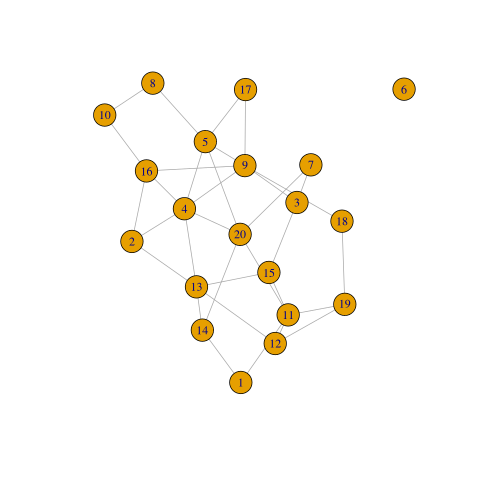
\includegraphics[width=.9\linewidth]{power-walk-example-graph.png}
\end{center}

\subsection{Using the Power Walk}
\label{sec:orgad46641}
\subsubsection{Inspect the newly created matrix and create constants}
\label{sec:org257ba2f}

\lstset{language=r,label= ,caption= ,captionpos=b,numbers=none}
\begin{lstlisting}
beta <- 0.843234
β    <- beta
n    <- nrow(A)

str(A)
\end{lstlisting}

\begin{verbatim}
Formal class 'dgCMatrix' [package "Matrix"] with 6 slots
  ..@ i       : int [1:504] 11 15 20 29 31 32 38 41 47 2 ...
  ..@ p       : int [1:51] 0 9 17 25 31 44 55 66 73 81 ...
  ..@ Dim     : int [1:2] 50 50
  ..@ Dimnames:List of 2
  .. ..$ : NULL
  .. ..$ : NULL
  ..@ x       : num [1:504] 1 1 1 1 1 1 1 1 1 1 ...
  ..@ factors : list()
\end{verbatim}

\subsubsection{Create a Diagonalised Scaling Matrix}
\label{sec:org008d6ab}
\lstset{language=r,label= ,caption= ,captionpos=b,numbers=none}
\begin{lstlisting}
sparse_diag <- function(mat) {
  #' Diagonal Factors of Sparse Matrix
  #'
  #' Return a Diagonal Matrix containing either 1 / colsum() or 0 such that
  #' matrix multiplication with this matrix would have all columns
  #' sum to 1
  #'
  #' This should take the transpose of an adjacency matrix in and the output
  #' can be multiplied by the original matrix to scale it to 1.
  #' i
  # mat  <- A
  ## Get the Dimensions
  n <- nrow(mat)

  ## Make a Diagonal Matrix of Column Sums
  D <- sparseMatrix(i = 1:n, j = 1:n, x = colSums(mat), dims = c(n,n))

  ## Throw away explicit Zeroes
  D <- drop0(D)

  ## Inverse the Values
  D@x <- 1/D@x

  ## Return the Diagonal Matrix
  return(D)
}
\end{lstlisting}

\subsubsection{Weight the Edges}
\label{sec:orgd9e1c9e}
Make the edges weighted with some real value

\lstset{language=r,label= ,caption= ,captionpos=b,numbers=none}
\begin{lstlisting}
weight_adjMat <- function(adjMat) {
  #' Weight Adjacency Matrix
  #'
  #' Randomly weights an adjacency matrix so that terms
  #' are Real (as opposed to natural) values.
  A@x*rnorm(length(A@x), 0, 0.1)
}
\end{lstlisting}

\subsubsection{Create a Probability Transition Matrix}
\label{sec:org7be8b81}
\lstset{language=r,label= ,caption= ,captionpos=b,numbers=none}
\begin{lstlisting}
adj_to_probTrans <- function(wadjmat, beta) {
  #' Adjacency to Probability Transition Matrix
  #'
  #' Returns a probability transition matrix from an input adjacency matrix
  #'
  #' Transposes an input matrix and then scales each column to sum to 1.
  #' Implemented with the Matrix dgCMatrix class in mind however also
  #' has logic to deal with a base matrix.
  #
  #' @param wadjmat A weighted adjacency matrix, ideally of the class dgCMatrix
  #' or atleast of the class matrix.
  #' @param beta The probability of following an edge

  wadjmat <- t(wadjmat)    # transpose Assuming row->column (like igraph)
#  wadjmat  <- A; beta  <- 0.8

  if ("dgCMatrix" %in% class(wadjmat)) {

#    B     <- sparseMatrix(i = summary(wadjmat)$i, j = summary(wadjmat)$j, x = beta^wadjmat@x) # element wise exponentiation
#    Don't do this ^^ because it comes out with clipped off dimensions
    B     <- wadjmat
    B@x   <- beta^wadjmat@x    # Element Wise exponentiation
    D_in  <- sparse_diag(B)
    T = B %*% D_in
    return(T)

  } else if ("matrix" %in% class(wadjmat)) {
    print("WARNING: expected dgCMatrix but matrix detected")
    print("Attemptying to proceed anyway")
    for (i in ncol(wadjmat)) {
      #  wadjmat[, i] <- wadjmat[, i] / sum(wadjmat[, i])
    B     <- wadjmat
    B   <- beta^wadjmat    # Element Wise exponentiation
    D_in  <- sparse_diag(B)
    T = B %*% D_in
    return(as.matrix(T))
    }
    return(wadjmat)
  } else {
    print("ERROR: Require sparse wadjmatrix of class dgCWadjmatrix to")
  }
}

class(A)
(T <- adj_to_probTrans(A, beta = 0.843234))  %>% summary %>% head()
\end{lstlisting}

\begin{verbatim}
[1] "dgCMatrix"
attr(,"package")
[1] "Matrix"
50 x 50 sparse Matrix of class "dgCMatrix", with 504 entries
   i j         x
1 12 1 0.1111111
2 16 1 0.1111111
3 21 1 0.1111111
4 30 1 0.1111111
5 32 1 0.1111111
6 33 1 0.1111111
\end{verbatim}
\subsubsection{Implement the Power Method to find the Stationary Point}
\label{sec:org6e1153b}
\lstset{language=r,label= ,caption= ,captionpos=b,numbers=none}
\begin{lstlisting}
## ** Power Method
p    <- rep(0, nrow(T))
p[1] <- 1
p_new    <- rep(0, nrow(T))
p_new[2]    <- 1

while (sum(round(p, 9) != round(p_new, 9))) {
    p     <- p_new
    p_new <- T %*% p
}



print(paste("The stationary point is"))
p %>% head()
\end{lstlisting}

\begin{verbatim}
[1] "The stationary point is"
6 x 1 Matrix of class "dgeMatrix"
           [,1]
[1,] 0.01785714
[2,] 0.01587302
[3,] 0.01587302
[4,] 0.01190476
[5,] 0.02579365
[6,] 0.02182540
\end{verbatim}
\subsection{Using Sparse Matrices}
\label{sec:orgbc166e7}
\subsubsection{Theory}
\label{sec:org56c7320}
if I have:

\begin{itemize}
\item \(\mathbf{O}_{i, j} := 0, \quad \forall i,j\leq n \in \mathbb{Z}^+\)

\item \(\vec{p_i}\) as the state distribution, being a vector of length \(n\)
\end{itemize}

Then it can be shown (see \eqref{eq:sparse-power-walk}):

$$\begin{aligned}
    \mathbf{O} \mathbf{D}_{\mathbf{B}}^{-1} \vec{p_i} = \mathtt{repeat} (\vec{p} \bullet \vec{\delta^{\tiny \mathrm{T}}} \mathtt{, n}\end{aligned})$$
where:

\begin{itemize}
\item \(\vec{\delta_i} = \frac{1}{\mathtt{colsums} \left( \mathbf{B} \right)}\)
\end{itemize}

This means we can do:

$$\begin{aligned}
     \vec{p_{i +  1}} &=  \mathbf{B} \mathbf{D}_{\mathbf{B}}^{- 1} \vec{p_{i}}  \\
     &= \left( \mathbf{B} -  \mathbf{O} +  \mathbf{O} \right) \mathbf{D}_{\mathbf{B}}^{- 1}\vec{p_i} \\
     &= \left( \left( \mathbf{B} -  \mathbf{O} \right) \mathbf{D}_{\mathbf{B}}^{- 1} +  \mathbf{O}\mathbf{D}_{\mathbf{B}}^{- 1} \right) \vec{p_i} \\
     &= \left( \mathbf{B}-  \mathbf{O}\right) \mathbf{D}_{\mathbf{B}}^{- 1} \vec{p_i} +  \mathbf{O} \mathbf{D}_{\mathbf{B}}^{- 1} \vec{p_i}  \\
     &= \left( \mathbf{B}- \mathbf{O} \right)\mathbf{D}_{\mathbf{B}}^{- 1} \vec{p_i} +  \vec{\delta'}\vec{p_i} \vec{1}
 \end{aligned}$$

And so the the power method can be implemented using sparse matrices.

\begin{enumerate}
\item Solving the Background Probability
\label{sec:org4060b28}
Define \(\vec{\delta}\) as the column sums of
\[\begin{aligned}
     \vec{\delta} & = \mathtt{colsum} (\text{{\bfseries{B}}})^{- 1}\\
     & = \frac{1}{\overrightarrow{1^{{\scriptsize \ensuremath{\boldsymbol{T}}}}}
     \ensuremath{\boldsymbol{B}}}
   \end{aligned}\]



\begin{align}
     \mathbf{OD}_{\mathbf{B}}^{- 1} \overrightarrow{p_i} & = \left(
     \begin{array}{cccc}
       1 & 1 & 1 & \\
       1 & 1 & 1 & \ldots\\
       1 & 1 & 1 & \\
       & \vdots &  & \ddots
     \end{array} \right) \left( \begin{array}{cccc}
       \delta_1 & 0 & 0 & \\
       0 & \delta_2 & 0 & \ldots\\
       0 & 0 & \delta_3 & \\
       0 & \vdots & 0 & \ddots
     \end{array} \right) \left( \begin{array}{c}
       p_1\\
       p_2\\
       p_3\\
       \vdots
     \end{array} \right) \nonumber \nonumber \\
     & = \left( \begin{array}{cccccc}
       \frac{p_1}{\delta 1} & + & \frac{p_2}{\delta_2} & + &
       \frac{p_3}{\delta_3} & \\
       \frac{p_1}{\delta 1} & + & \frac{p_2}{\delta_2} & + &
       \frac{p_3}{\delta_3} & \ldots\\
       \frac{p_1}{\delta 1} & + & \frac{p_2}{\delta_2} & + &
       \frac{p_3}{\delta_3} & \\
       &  & \vdots &  &  & \ddots
     \end{array} \right) \nonumber \nonumber \\
     & = \left(\begin{array}{c}
       \sum^n_{i = 1} [p_{_i} \delta_i]\\
       \sum^n_{i = 1} [p_{_i} \delta_i]\\
       \sum^n_{i = 1} [p_{_i} \delta_i]\\
       \vdots
     \end{array}\right) \nonumber \\
     & = \left( \begin{array}{c}
       \overrightarrow{\delta^{\tiny{\ensuremath{\boldsymbol{T}}}}} \bullet \vec{p}\\
       \overrightarrow{\delta^{\tiny{\ensuremath{\boldsymbol{T}}}}} \bullet \vec{p}\\
       \overrightarrow{\delta^{\tiny{\ensuremath{\boldsymbol{T}}}}} \bullet \vec{p}\\
       \vdots
     \end{array} \right) \nonumber \\
     & = \mathtt{repeat} (\vec{p} \bullet \vec{\delta^{\tiny \mathrm{T}}} \mathtt{, n}) \label{eq:sparse-power-walk}
   \end{align}
\end{enumerate}
\subsubsection{Set the value for B}
\label{sec:org382933d}
\lstset{language=r,label= ,caption= ,captionpos=b,numbers=none}
\begin{lstlisting}
B     <- A
B@x   <- β^(A@x) -1
\end{lstlisting}

\subsubsection{Create the Scaling Matrix}
\label{sec:orgc9b32d0}
The Transition probability matrix must sum to 1 so use the scaling matrix reduce
the column sums.

\lstset{language=r,label= ,caption= ,captionpos=b,numbers=none}
\begin{lstlisting}
δB   <- 1/colSums(B)
δBt  <- t(δB)
DB   <- diag(δB)
\end{lstlisting}

\subsubsection{Create the Trans Prob Mat}
\label{sec:orgdb41a7a}
\lstset{language=r,label= ,caption= ,captionpos=b,numbers=none}
\begin{lstlisting}
T <- B %*% DB
\end{lstlisting}

\subsubsection{Implement the Power Walk}
\label{sec:org062cf81}
\begin{enumerate}
\item Set the Starting Values
\label{sec:orgeaa690e}
\lstset{language=r,label= ,caption= ,captionpos=b,numbers=none}
\begin{lstlisting}
p_new  <- rep(1/n, n)  # Uniform
p      <- rep(0, n)    # Zero
η      <- 10^(-6)
\end{lstlisting}

\item Implement the loop
\label{sec:org1a46e7c}
\lstset{language=r,label= ,caption= ,captionpos=b,numbers=none}
\begin{lstlisting}
while (sum(abs(p_new - p)) > η) {
(p <- as.vector(p_new)) # P should remain a vector
sum(p <- as.vector(p_new)) # P should remain a vector
    p_new  <- T %*% p + rep(δBt %*% p, n)
}
\end{lstlisting}

\begin{verbatim}
Error in while (sum(abs(p_new - p))
η) { :
  missing value where TRUE/FALSE needed
\end{verbatim}


This error results because the \(\vec{p_{i}} \rightarrow \infty\)

\item Print the Stationary value
\label{sec:org5bcec24}
\lstset{language=r,label= ,caption= ,captionpos=b,numbers=none}
\begin{lstlisting}
p %>% head()
\end{lstlisting}

\begin{verbatim}
[1] -Inf -Inf -Inf -Inf -Inf -Inf
\end{verbatim}
\end{enumerate}
\end{document}
